\section{Methods}\label{meth}
We conceptualize bias adjustments to aggregate estimates of
duration selling sex and partnership change rates
using Bayesian hierarchical models.
We then attempt to infer unbiased estimates of these parameters
via Gibbs sampling \cite{Geman1984}.
Implementation details are given in Appendix~\ref{app.code}.
We use data from \cite{Baral2014}, in which 328 women aged 15+
who reported exchanging or selling sex for money, favors, or goods in the past 12 months
were recruited via respondent-driven sampling (RDS) \cite{Heckathorn1997}.
\begin{figure}
  \begin{subfigure}[b]{\textwidth}
    \centering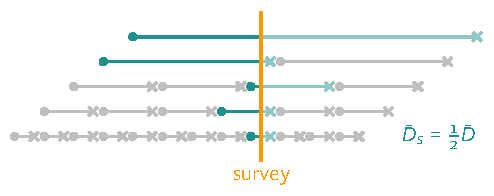
\includegraphics[scale=1]{diag.yss.censor}
    \caption{Right censoring of reported durations selling sex in a steady state population}
    \label{fig:diag.yss.censor}
  \end{subfigure}
  \begin{subfigure}[b]{\textwidth}
    \centering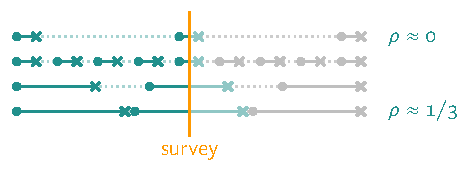
\includegraphics[scale=1]{diag.yss.gaps}
    \caption{Possible periods of selling sex for one respondent who stopped 0, 1, or 2 times}
    \label{fig:diag.yss.gaps}
  \end{subfigure}
  \begin{subfigure}[b]{\textwidth}
    \centering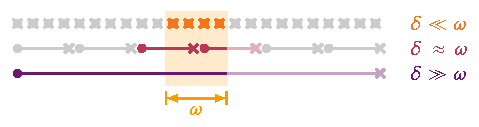
\includegraphics[scale=1]{diag.partner.cases}
    \caption{Differences in partnership duration \vs recall period}
    \label{fig:diag.partner.cases}
  \end{subfigure}
  \begin{subfigure}[b]{\textwidth}
    \centering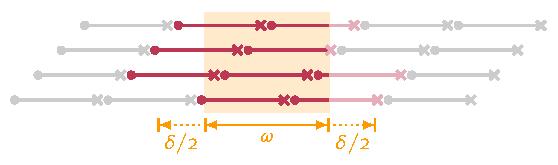
\includegraphics[scale=1]{diag.partner.recall}
    \caption{Fully and partially observed partnerships during a given recall period}
    \label{fig:diag.partner.recall}
  \end{subfigure}
  \caption{Diagrams of fully observed, censored, and unobserved periods
    selling sex or within ongoing sexual partnerships}
  \label{fig:diag}
  \floatfoot{Guide:
    \g{$\bullet$\,}{start}, \g{$\bm{\times}$\,}{end},
    \g{yellow}{survey/recall period},
    \g{full colour}{fully observed}, \g{faded colour}{right censored}, \g{grey}{unobserved},
    \g{$\bar{d}$}{mean duration at survey} and \g{$\bar{D}$}{overall},
    \g{$s$}{number of times stopped selling sex}, \g{$g$}{relative gap length \vs $D$},
    \g{$\omega$}{recall period}, \g{$\delta$}{partnership duration},
    \g{$x$}{number of reported partnerships}.}
\end{figure}
%===================================================================================================
\subsection{Duration Selling Sex}\label{meth.yss}
%---------------------------------------------------------------------------------------------------
\paragraph{Crude Estimates}
The survey \cite{Baral2014} included questions about
the current respondent's age and the age of first selling sex.
The difference between these ages could be used to define a crude ``duration selling sex''.
Using this approach, the crude median duration was $\tilde{d} = 4$ years.
However, if durations are assumed to be exponentially distributed
--- a implicit assumption in compartmental models \cite{Anderson1991} ---
then the crude mean could be estimated from the crude median as
$\bar{d} = \tilde{d}/\distr{log}{2}$ due to skewness.
To move beyond crude estimates, next we develop the hierarchical model,
% SM: maybe explain or reference "generative model" [to reach a more general epi audience]?
%     (eg. "...to produce a representation or abstraction of the observed phenomena
%     that could be calculated from the observations)...
% JK: reading up on this, I think 'generative' (my understanding: we can generate new random data from it)
%     is basically redundant with 'Bayesian' here, so I've removed 'generative' throughout,
%     and updated to consistently describe the models as
%     'Bayesian hierarchical models' or 'hierarchical model' in a few places for brevity
considering the following potential biases.
%---------------------------------------------------------------------------------------------------
\paragraph{Sampling}
Sampling bias was considered via RDS-adjustment in \cite{Baral2014},
yielding mean and \ci estimates of the proportions of respondents $p_z$
who had sold sex starting $\mathbb{d}_z \in \{0{-}2, 3{-}5, 6{-}10, 11+\}$ years ago
(Table~\ref{tab:data}, ``$z$'' enumerates strata).
% The adjusted proportions indicate fewer years selling sex \vs the unadjusted proportions,
% which would be consistent with challenges in reaching women in the first year(s) of sex work \cite{Roberts2020}.
% SM: agree with moving above to discussion
%     [can cite Elizabeth's Kenya paper as an example and/or HM's CROI abstract - access gap paper not yet in preprint ugh].
% JK: As it is, this doesn't really fit anywhere in the discussion,
%     and might be a bit distracting from the methods focus.
%     I've left it out for now and see whether reviewers ask
%     for more comment on the results in context.
We start by defining a model to identify distributions of reported durations $d_i$
which are consistent with these data.
We model each proportion $p_z$ as a random variable with
a beta approximation of binomial (BAB) distribution (see Appendix~\ref{app.bab})
with parameters $N_z$ and $\rho_z$.
We model each $N_z$ as a fixed value,
which we fit to the \ci of $p_z$ as described in \sref{app.bab}.
We then model each $\rho_z$ as
the proportion of reported durations $d_i$ within the interval $\mathbb{d}_z$.
Since these proportions are difficult to define analytically,
we estimate $\hat{\rho}_z = \distr{mean}{d_i \in \mathbb{d}_z}$ from $N = 100$ samples.
%---------------------------------------------------------------------------------------------------
\paragraph{Censoring}
These reported durations $d_i$ are effectively right censored
because they only capture engagement in sex work up until the survey, and
and not additional sex work after the survey
(Figure~\ref{fig:diag.yss.censor}) \cite{Fazito2012}.
If we assume that the survey reaches respondents at a random time point
during their total (eventual) duration selling sex $D_i$, we can model this censoring via
a random fraction $f_i \sim \distr{Unif}{0,1}$, such that $d_i = f_i D_i$.
The expected means are then related by $\bar{d} / \bar{D} = \bar{f} = \frac12$.
%---------------------------------------------------------------------------------------------------
\paragraph{Measurement}
Finally, respondents may not sell sex continuously.
% SM: optional edit - paranthesis example not needed but may want to relate back to the intro ... see what you think
%     (i.e. enter, exit, and re-enter periods/seasons of occupational risk)
% JK: It might be a bit distracting re. the flow of ideas grounded in the example
Reported durations $d_i$ may therefore include
multiple periods of selling sex with gaps in between,
whereas we aim to model $D_i$ as the durations of individual periods selling sex.
Respondents in \cite{Baral2014} were not asked whether they ever temporarily stopped selling sex,
% SM: "cease" may be a better term than "stopped"?;
%     and presuming this survey asked about temporarily cessastion of sex work?
% JK: I might be missing the nuance, but 'stop' and 'cease' seem interchangeable?
%     and 'stop' feels more accessible?
but a later survey \cite{EswKP2014} indicated that $\phi = 45\%$ had stopped at least once.
% SM: did they ask about duration of the periods in between engagement in sex work?
% JK: they didn't unfortunately -- but we can maybe ask BS re. the upcoming survey!
We model the number of times a respondent may temporarily stop selling sex as
a Poisson-distributed random variable $s_i$ with mean~$\bar{s}$.
The expected value of $\phi$ given $\bar{s}$ is then $\distr{P}{s > 0} = 1 - e^{-\bar{s}}$.
Since $\phi = 45\%$ is an imperfect observation,
we model $\phi$ as a random variable with a BAB distribution
having parameters $N = 328$ and $\rho = 1 - e^{-\bar{s}}$,
which allows inference on $\bar{s}$ given $\phi$.
\par
Next, we update the model for reported durations as $d_i = D_i\,(f_i + s_i\,(1 + g_i))$,
where $g_i$ is the relative duration of gaps between selling sex,
with the following rationale.
If $s_i = 0$, then $d_i = f_i D_i$ as before, reflecting the censored current period only.
If $s_i > 0$, then $d_i$ also includes $s_i$ prior periods selling sex and the gaps between them
(Figure~\ref{fig:diag.yss.gaps}) --- \ie $s_i\,(D_i + g_i D_i) = D_i\,s_i\,(1 + g_i)$.
The major assumption we make here is that
all successive periods are of equal length, and likewise for gaps between them.
We must also assume a distribution for $g_i$, for which we choose
$g_i \sim \distr{Exp}{1/\bar{g}}$, arbitrarily.
%---------------------------------------------------------------------------------------------------
\paragraph{Summary}
Figure~\ref{fig:model.yss} summarizes the proposed model graphically.
The primary parameter of interest is
the mean duration selling sex (for a given period) $\bar{D}$,
but we must also infer
the mean number of times respondents stop selling sex $\bar{s}$, and
the mean relative duration of gaps $\bar{g}$.
We assume uninformative priors for these 3 parameters.

%---------------------------------------------------------------------------------------------------
\begin{figure}
  \begin{subfigure}{\textwidth}
    \begin{minipage}{.5\textwidth}
      \centering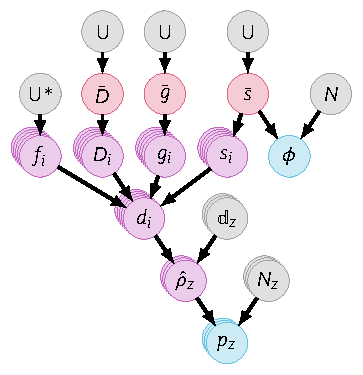
\includegraphics[scale=1]{model.yss}
    \end{minipage}
    \begin{minipage}{.5\textwidth}
      \begin{subequations}
      \begin{align}
           p_z &\sim \distr{BAB}{N_z, \hat{\rho}_z} \\
  \hat{\rho}_z &=    \distr{mean}{d_i \in \mathbb{d}_z} \\
           d_i &=    D_i\,(f_i + s_i\,(1 + g_i)) \\
           D_i &\sim \distr{Exp}{1/\bar{D}} \\
           f_i &\sim \distr{Unif}{0,1} \\
           s_i &\sim \distr{Pois}{\bar{s}} \\
           g_i &\sim \distr{Exp}{1/\bar{g}} \\
          \phi &\sim \distr{BAB}{N, 1-e^{-\bar{s}}\,}
      \end{align}
      \end{subequations}
    \end{minipage}
    \caption{Duration selling sex}
    \label{fig:model.yss}
  \end{subfigure}
  \begin{subfigure}{\textwidth}
    \begin{minipage}{.5\textwidth}
      \centering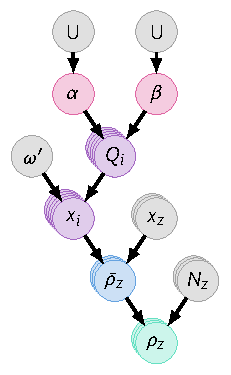
\includegraphics[scale=1]{model.part}
    \end{minipage}
    \begin{minipage}{.5\textwidth}
      \begin{subequations}
      \begin{align}
           p_z &\sim \distr{BAB}{N_z, \hat{\rho}_z} \\
  \hat{\rho}_z &=    \distr{mean}{x_i \in \mathbb{x}_z} \\
           x_i &\sim \distr{Pois}{Q_i\,\omega'} \\
           Q_i &\sim \distr{Gamma}{\alpha,\beta}
      \end{align}
      \end{subequations}
    \end{minipage}
    \caption{Rates of partnership change}
    \label{fig:model.part}
  \end{subfigure}
  \captionall{Graphical and mathematical representations
    of the proposed Bayesian hierarchical models}
  \label{fig:model}
  \floatfoot{Guide:
    \g{gray}{fixed variable/distribution},
    \g{red}{target},
    \g{purple}{intermediate},
    \g{blue}{observed}.
    Variables:
    % both
    \g{$p_z$}{proportion of population},
    \g{$N_z$}{effective sample size},
    \g{$\hat{\rho}_z$}{empirically estimated $p_z$ mean},
    % yss
    \g{$\mathbb{d}_z$}{range of reported durations selling sex},
    \g{$d_i$}{reported duration at survey},
    \g{$D_i$}{total (eventual) duration},
    \g{$f_i$}{censoring fraction},
    \g{$s_i$}{number of times stopped selling sex},
    \g{$g_i$}{relative gap length},
    \g{$\bar{D}$}{true $D$ mean},
    \g{$\bar{s}$}{true $s$ mean},
    \g{$\bar{g}$}{true $g$ mean},
    \g{$\phi$}{proportion who stopped selling sex at least once},
    % parts
    \g{$\mathbb{x}$}{range of reported partner numbers},
    \g{$x_i$}{reported partner numbers},
    \g{$Q_i$}{partnership change rate},
    \g{$\omega'$}{effective recall period},
    \g{$\alpha,\beta$}{parameters of $Q_i$ distribution}.
    % misc
    Distributions:
    \g{U}{uniform / uninformative},
    \g{BAB}{beta approximation of binomial distribution}.
  }
\end{figure}

%===================================================================================================
\subsection{Rates of Partnership Change}\label{meth.parts}
%---------------------------------------------------------------------------------------------------
\paragraph{Base Data \& Assumptions}
The survey \cite{Baral2014} also asked respondents to report
their numbers of sexual partners ($x$) in a recall period ($\omega$) of $30$ days.
Numbers were stratified by three types of partner:
new paying clients, regular paying clients, and non-paying partners.
We assume that only a small proportion of new clients go on to become regular clients;
thus, we conceptualize ``new'' clients as effectively ``one-off'' clients.%
\footnote{The number of new clients per recall period
  could also be used to define a rate of partnership change \cite{Fazito2012},
  but we do not explore this approach here.}
Since no survey questions asked about partnership durations ($\delta$),
we further assume that these were:
1~day with new paying clients,
4~months with regular paying clients, and
3~years with non-paying partners.
We now develop the hierarchical model to estimate
the expected rate of partnership change for each type,
considering the following potential biases.
%---------------------------------------------------------------------------------------------------
\paragraph{Sampling}
As before, \cite{Baral2014} estimates RDS-adjusted proportions of respondents $p_z$ (mean, \ci)
reporting different numbers/ranges of partners $\mathbb{x}_z$ in the past 30 days
(Table~\ref{tab:data}).
Thus, we take the same approach as in \sref{meth.yss}
to identify distributions of reported partner numbers $x_i$
which are consistent with these proportion data for each partnership type.
%---------------------------------------------------------------------------------------------------
\paragraph{Duration Assumptions}
Numbers of reported partners ($x$) have generally been interpreted in two ways ---
$x/\omega$ as the \emph{rate} of partnership change ($Q$) or
$x$ as the \emph{number} of current partners ($K$):
\begin{subequations}\label{eq:bQK}
\begin{alignat}{1}
  Q &\approx \frac{x}{\omega} \label{eq:bQ}\\
    &\text{or} \nonumber\\
  K &\approx x \label{eq:bK}
\end{alignat}
\end{subequations}
Both interpretations are reasonable under certain conditions:
If partnership duration is short and the recall period is long
($\delta \ll \omega$, \eg 1~day \vs 1~month),
then reported partnerships mostly reflect \emph{complete} partnerships,
and thus $x/\omega \approx Q$.
If partnership duration is long and the recall period is short
($\delta \gg \omega$, \eg 1~year \vs 1~month),
then reported partnerships mostly reflect \emph{ongoing} partnerships,
and thus $x \approx K$.
However, if partnership duration and recall period are similar in length
($\delta \approx \omega$, \eg 1~month \vs 1~month),
then reported partnerships reflect a mixture of tail-ends, of complete, and of ongoing partnerships.
Thus $x/\omega$ overestimates $Q$, but $x$ also overestimates $K$.
These three cases are illustrated in Figure~\ref{fig:diag.partner.cases}.
\par
To adjust for this bias, we again assume that survey/recall period timing is effectively random.
Then, if the \emph{end} of the recall period would intersect an ongoing partnership,
then a random fraction $f_i \sim \distr{Unif}{0,1}$ of the partnership duration $\delta$
would be outside the recall period.
As before, the expected value $\bar{f} = \frac12$.
The same goes for the \emph{start} of the recall period.
Thus, the recall period is effectively extended by
half the partnership duration $\delta/2$ on each end, and $\delta$ overall \cite{Neely2023},
as illustrated in Figure~\ref{fig:diag.partner.recall}.
We can therefore define unbiased estimators of $Q$ and $K$ as:
\begin{subequations}\label{eq:uQK}
\begin{alignat}{1}
  Q &= \frac{x}{\omega + \delta}\\
  K &= \frac{x \delta}{\omega + \delta} = Q \delta
\end{alignat}
\end{subequations}
To apply \eqref{eq:uQK} in the hierarchical model, we sample the true rate of partnership change
from an assumed distribution $Q_i \sim \distr{Gamma}{\alpha,\beta}$,
with unknown parameters $\alpha, \beta$.
Then, we model the numbers of reported partners $x_i$
given $Q_i$ and $\omega' = (\omega + \delta)$ as: $x_i \sim \distr{Poi}{Q\,\omega'}$.
%---------------------------------------------------------------------------------------------------
\paragraph{Summary}
Figure~\ref{fig:model.part} summarizes the proposed model graphically.
The primary parameters of interest are $\alpha, \beta$, which govern
the distribution of rates of partnership change (for a given type) $Q$.
We assume uninformative priors for these 2 parameters.
%---------------------------------------------------------------------------------------------------
\paragraph{Comparing Assumptions}
To quantify the influence of using
the biased \vs unbiased estimators of $Q$ and $K$,
we fit the proposed model for each partnership type under three assumptions:
assuming \emph{short} partnerships as in \eqref{eq:bQ} with $\omega' = \omega$;
assuming \emph{long} partnerships as in \eqref{eq:bK} with $\omega' = \delta$; and
our \emph{unbiased} approach as in \eqref{eq:uQK} with $\omega' = \omega + \delta$.
To illustrate more general trends in the magnitude of bias,
we further compared biased \vs unbiased estimates of $Q$ and $K$ across a range of different
partnership durations $\delta \in [0.1, 10]$ and
recall periods $\omega \in [0.1, 10]$,
with fixed true rate $Q = 1$ (arbitrary units).

